\section{Automates finis et langages}

\subsection{Mots et langages}

Avant de nous intéresser à proprement parler aux automates ou autres machines, nous allons devoir formaliser ce dont il sera question dans ce chapitre. En reprenant ce qui a été dit plus tôt, il nous faut formaliser la notion d'objet, et celle de propriété sur un objet. En théorie des ensembles, un objet est simplement un ensemble comme un autre, et une propriété sur un ensemble est simplement une propriété du calcul des prédicats comme nous l'avons vu. Mais d'un point de vue d'informaticien, un objet est en général codé, et c'est ce point de vue que nous allons adopter. Nous allons donc nous intéresser, comme objets, à des \og codes d'objets\fg{}, qui seront plus précisément des mots :

\begin{defi}[Mot sur un alphabet]
    Soit $\Sigma$ un ensemble fini non vide que l'on appellera alphabet. On dit que $u$ est un mot sur $\Sigma$ si $u$ est une suite finie d'éléments de $\Sigma$, c'est-à-dire qu'il existe $n$ tel que $u\in\Sigma^n$. L'ensemble des mots sur $\Sigma$ est noté $\Sigma^*$, et est donc défini par $$\Sigma^*=\bigcup_{n\in \nat} \Sigma^n$$ en prenant la convention que $\Sigma^0 = \{\varepsilon\}$ où $\varepsilon$ est appelé le mot vide. Pour un mot $u\in \Sigma^*$, on appellera sa longueur l'entier $n$ tel que $u\in\Sigma^n$, et on la notera $|u|$. De plus, on notera $u_i$ pour la $i$\ieme{} composante du mot $u$.
\end{defi}

\begin{rmk}
    Par convention, les indices vont de $0$ à $|u|-1$.
\end{rmk}

\begin{expl}
    Soit l'alphabet $\Sigma=\{0,1\}$. Un mot sur $\Sigma$ est par exemple $0010$ (on notera ainsi, plutôt que $(0,0,1,0)$, les mots).
\end{expl}

Notre formalisme repose donc sur l'étude des mots. Nous allons donc définir l'opération essentielle sur les mots.

\begin{defi}[Concaténation]
    On définit l'opération de concaténation, qui à un mot $u$ et un mot $v$ associe le mot $u\cdot v$ défini par $$(u\cdot v)_i =\left\{\begin{array}{ll} u_i & \mbox{si}\; i<|u| \\ v_{|u|-i} & \mbox{sinon.} \end{array}\right.$$

    Cette opération est définie pour tous $n,m\in\nat$ comme $\cdot : \Sigma^n\times \Sigma^m \to \Sigma^{n+m}$ et peut donc directement se prolonger en une loi de composition interne sur $\Sigma^*$.
\end{defi}

\begin{expl}
    Toujours sur l'alphabet $\Sigma= \{0,1\}$, la concaténation nous donne $0010\cdot 100 = 0010100$.
\end{expl}

\begin{exo}[Les mots forment un monoïde]
    Montrer que $\cdot$ est une loi associative, c'est-à-dire que $(u\cdot v)\cdot w = u\cdot (v\cdot w)$ pour tous $u,v,x\in\Sigma^*$. Montrer de plus que $\varepsilon$ est neutre pour $\cdot$, c'est-à-dire que $u\cdot\varepsilon = \varepsilon \cdot u = u$ pour tout $u\in\Sigma^*$.
\end{exo}

\begin{rmk}
    On aurait pu définir l'ensemble des mots sur $\Sigma$ de façon plus algébrique en considérant ce qu'on appelle le monoïde libre sur $\Sigma$, mais ça n'est pas le point de vue le plus adapté dans notre étude actuelle car nous ne parlerons pas de morphisme de monoïde.
\end{rmk}

Nous en venons maintenant à chercher comment définir une propriété sur ces mots : la façon la plus naturelle est de regarder tous les mots vérifiant la propriété, d'où la définition suivante :

\begin{defi}[Langage]
    On appelle un langage sur $\Sigma$ une partie $L\subseteq\Sigma^*$. C'est donc un ensemble de mots, et on peut le voir comme la description d'une propriété : au lieu de dire qu'un mot $u$ a une certaine propriété $P$, on associera à $P$ un langage $L$ et on dira directement que $u\in L$.
\end{defi}

Nous allons maintenant définir les opérations basiques associées aux langages :

\begin{defi}[Opérations sur les langages]
    Soient $L$ et $L'$ deux langage. On définit les opérations suivantes :
    \begin{itemize}[label=$\bullet$]
        \item $L\cdot L' = \{ u\cdot v \mid u\in L, v \in L'\}$
        \item $L\cup L'$ que l'on notera souvent $L + L'$.
        \item $L^n$ défini par $L^0 = \{\varepsilon\}$ et $L^{n+1} = L\cdot L^n$.
        \item $L^* = \displaystyle{\bigcup_{n\in\nat}L^n}$
        \item $L^c = \Sigma^* \setminus L$
    \end{itemize}
\end{defi}

\begin{expl}
    Soit $L = \{0,01\}$ et $L' = \{\varepsilon,100\}$, alors $L\cdot L' = \{0,01,0100,01100\}$, $L+L' = \{0,01,\varepsilon,100\}$, $L^c$ est l'ensemble des mots qui ne sont ni $0$ ni $01$ et $L^*$ est l'ensemble des mots qui s'écrivent $u_1\cdot u_2\cdots u_p$ où $u_i\in L$ pour $1\leq i \leq p$, par exemple $0010001 = 0\cdot 01 \cdot 0\cdot 0 \cdot 01 \in L^*$.
\end{expl}

\subsection{Définition d'un automate déterministe et indéterministe}

Intuitivement, donnons-nous le langage $L$ sur $\{0,1\}$ des mots qui sont une alternance de $0$ et de $1$. Quel procédé pourrions-nous trouver, étant donné un mot $u$, pour savoir si $u\in L$ ? Par procédé nous cherchons un objet mathématique qui pourrait trier pour nous les mots appartenant à $L$ ou non. Dans cette section, nous nous intéresserons à la construction la plus basique de ces objets, appelés automates. Les automates prennent donc un mot en entrée et, par une successions d'actions (définies purement mathématiquement) répondent si le mot est dans le langage $L$ ou non. La première approche est de considérer le mot lettre par lettre, et de \og lire\fg{} linéairement le mot, en stockant une information au maximum à la lecture du mot. Cela nous mène à la définition suivante :

\begin{defi}[Automate fini déterministe]
    Soit $\Sigma$ un alphabet, un automate $\aA$ est la donnée d'un quintuplet $(\Sigma,Q,q_0,\delta,F)$ où :
    \begin{itemize}[label=$\bullet$]
        \item $\Sigma$ est l'alphabet sur lequel on travaille.
        \item $Q$ est un ensemble d'états fini non vide.
        \item $q_0 \in Q$ est l'état initial de l'automate.
        \item $\delta : \Sigma \times Q \to Q$ est la fonction de transition (considéré partielle), disant après la lecture d'une lettre dans quel état doit se rendre l'automate.
        \item $F\subseteq Q$ est l'ensemble des états finaux.
    \end{itemize}
\end{defi}

Si la définition peut faire peur, elle revient généralement à dessiner un graphe où les états sont les sommets et les arcs (orientés) sont étiquetés par des lettres. On note une flèche entrante pour désigner l'état initial, et on entoure en double les états finaux. Nous donnons une présentation d'un automate dans la figure \ref{fig:automate1} suivante :

\begin{figure}[h]
    \centering
    \rule{17cm}{0.5pt}\\
    \vspace{0.5cm}
    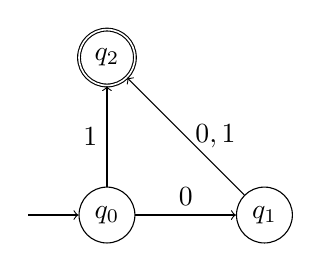
\begin{tikzpicture}
\node[draw,circle] (A) at (0,0) {$q_0$};
\draw[->] (-1,0) -- (A);
\node[draw,circle] (B) at (2,0) {$q_1$};
\node[draw,double,circle] (C) at (0,2) {$q_2$};
\draw[->] (A) -- (B);
\draw (1,0) node [above] {$0$};
\draw[->] (B) -- (C);
\draw (1,1) node [above,right] {$0,1$};
\draw[->] (A) -- (C);
\draw (0,1) node [left] {$1$};
\end{tikzpicture}
    \rule{17cm}{0.5pt}\\
    \vspace{0.5cm}
    \caption{Un automate $\aA_0$.}
    \label{fig:automate1}
\end{figure}

On a donc $\Sigma = \{0,1\}$, $Q=\{q_0,q_1,q_2\}$, $F=\{q_2\}$ et la fonction de transition décrite par \begin{align*}
    \delta (0,q_0) &= q_1\\
    \delta (1,q_0) &= q_2\\
    \delta (0,q_1) &= q_2\\
    \delta (1,q_1) &= q_2\\
    \delta (\alpha,q_2) &= \bot
\end{align*}
 où $\bot$ signifie que la fonction n'est pas définie sur ce couple.

 On remarque rapidement que si l'on arrive à un état, on peut appliquer à nouveau la fonction de transition depuis cet état si l'on a une nouvelle lettre : ce sera le fonctionnement de notre automate, qui prendra en entrée un mot et, à chaque lettre, appliquer la fonction de transition une fois pour passer de l'état initial à un certain état, et il acceptera le mot suivant si l'état atteint par ce procédé est ou non un état final. Un état sera donc principalement vu comme une machine opérant sur les mots, et caractérisant un langage, donc un ensemble de mots.

 \begin{defi}[Langage accepté par un automate déterministe]
     Soit $\aA$ un automate fini déterministe. On étend par récurrence la fonction de transition sur $\Sigma^*$ : \begin{itemize}[label=$\bullet$]
         \item $\delta^*(\varepsilon,q) = q$ pour tout état $q\in Q$
         \item $\delta^*(\alpha\cdot v,q) = \delta(\alpha,\delta^*(v,q))$ pour $\alpha$ une lettre et $v$ un mot.
     \end{itemize}

     On notera aussi, en général, $q\cdot u$ pour désigne $\delta^*(u,q)$, nous donnant dont $q\cdot (\alpha\cdot v) = (q\cdot \alpha)\cdot v$, ce qui est plus lisible.

     On dit que $\aA$ accepte un mot $u$ si $q_0\cdot u \in F$, et on note alors $\aA(u)=1$. Si $q_0\cdot u$ n'est pas défini (qu'on arrive sur une transition non définie, comme dans l'exemple avec $\bot$) ou que $q_0\cdot u \notin F$, on dit que $\aA$ rejette le mot $u$ et on note alors $\aA(u)=0$.

     On définit par $L(\aA)$ l'ensemble des mots acceptés par $\aA$ : $$L(\aA) =\{u\in \Sigma^*\mid \aA(u)=1\}$$
 \end{defi}

 De façon équivalente, qu'un mot $u$ soit accepté par $\aA$ peut s'écrire comme le fait qu'il existe une suite $q_0,\ldots,q_p$ où $q_p\in F$ et $q_{i+1}=\delta(q_i,u_i)$. Ces automates sont dits déterministes car cette suite est unique, lors de la lecture d'un mot. Nous allons donc introduire la notion d'automate non déterministe :

 \begin{defi}[Automate fini non déterministe]
     Un automate fini non déterministe est un quintuplet $(\Sigma,Q,Q_0,\delta,F)$ où $\Sigma,Q$ et $F$ sont identiques au cas déterministe, mais $Q_0\subseteq Q$ et $\delta : \Sigma \times Q \to \mathcal P(Q)$. Le changement sur $Q_0$ signifie simplement que l'on s'autorise plusieurs états initiaux, mais le changement sur delta mérite plus d'explications : l'image d'une transition est un ensemble d'états, on peut voir cela comme \og les états qui peuvent arriver après la transition \fg{}.
 \end{defi}

 On peut ensuite définir ce qu'est le langage reconnu par un automate non déterministe :

 \begin{defi}
     Soit $\aA$ un automate non déterministe, on dit que $u$ est reconnu par $\aA$ s'il existe une suite $q_0,\ldots,q_p$ où $q_0\in Q_0$, $q_{i+1}\in \delta(u_i,q_i)$ et $q_p\in F$.

     On peut alors définir de façon analogue le langage reconnu par $\aA$, que l'on notera $L(\aA)$.
 \end{defi}

 Les automates non déterministes sont beaucoup plus pratiques à manipuler, mais leur expressivité est la même que les automates déterministes :

 \begin{them}
    Soit $L$ un langage sur un alphabet $\Sigma$. $L$ est le langage reconnu par un automate déterministe si et seulement s'il est le langage reconnu par un automate non déterministe.
 \end{them}

 \begin{proof}
    Un des sens est évident : on peut facilement transformer un automate déterministe en un automate non déterministe en fixant $Q_0=q_0$ et $\delta'(\alpha,q) = \{q\cdot \alpha\}$.

    Nous allons donc prouver le sens réciproque : soit $\aA$ non déterministe dont le langage reconnu est $L$, construisons $\aA'$ déterministe tel que $L(\aA) = L(\aA')$. En notant $\aA = (\Sigma,Q,Q_0,\delta,F)$ on va construire notre automate $\aA' = (\Sigma,Q',q_0,\delta',F')$ de la façon suivante :
    \begin{itemize}[label=$\bullet$]
        \item $Q'=\mathcal P(Q)$ : l'ensemble des états de $\aA'$ est l'ensemble des parties des états de $\aA$.
        \item $q_0 = Q_0$ puisque $Q_0\in \mathcal P(Q)$.
        \item $\delta'(\alpha,p) = \displaystyle{\bigcup_{q\in p}\delta(\alpha,q)}$
        \item $F' = \{P\subseteq Q\mid P\cap F \neq \varnothing\}$
    \end{itemize}

    Montrons qu'alors $\aA(u) = \aA'(u)$ :
    \begin{itemize}[label=$\bullet$]
        \item Supposons que $\aA$ reconnaisse $u$, alors il existe une suite $q_0,\ldots,q_p$ telle que $q_0\in Q_0$, pour chaque $i$ $q_{i+1}\in \delta(u_i,q_i)$ et $q_p\in F$. Dans $\aA'$, on remarque que chaque $q_i$ appartient à $\delta'^*(u_{<i},Q_0)$ (en notant $u_{<i}$ le préfixe de $u$ construit en prenant les $i$ premières lettres). En effet par hypothèse $q_0\in Q_0$, puis si $q_i\in \delta'^*(u_{<i},Q_0)$, en réécrivant $\delta'^*(u_{<i+1},Q_0)$, on obtient $$\delta'^*(u_{<i+1},Q_0) = \bigcup_{q \in \delta'^*(u_{<i},Q_0)} \delta(u_i,q)$$ mais comme $q_{i+1}\in \delta(u_i,q_i)$ on en déduit que $q_{i+1}\in \delta'^*(u_{<i+1},Q_0)$. Enfin, comme le dernier état $q_p$ est final, cela signifie que le dernier état de la lecture par $\aA'$ contient un état final, ce qui signifie que c'est un état final : on en déduit que $\aA'$ reconnaît $u$.
        \item Réciproquement, si $\aA'$ accepte un mot $u$, montrons qu'il en est de même pour $\aA$. Pour cela, on va montrer la réciproque de la propriété précédente : pour toute suite $Q_0,\ldots,Q_p$ où $Q_{i+1}=\delta'(u_i,Q_i)$ et tout élément $q_{k}\in Q_{k}$ il existe une suite $q_0,\ldots,q_k$ telle que $q_0\in Q_0$ et $q_{i+1}\in \delta(u_i,q_i)$. Le cas de base, avec $q_0$, est évident, passons donc à l'hérédité : prenons $q_{k+1}\in Q_{k+1}$, alors $Q_{k+1}=\delta'(u_k,Q_k)$ et par hypothèse de récurrence, $q_k\in Q_k$, et on remarque que $\delta'(u_k,Q_k)$ contient $\delta(u_k,q_k)$ (puisque c'est l'un des termes de l'union), donc $q_{k+1}\in Q_{k+1}$. Par hypothèse, $\aA'$ accepte $u$, ce qui signifie qu'il existe $q_f\in Q_p$ tel que $q_f \in F$, donc par le résultat que l'on vient de montrer, il existe un chemin acceptant dans $\aA'$, donc $\aA'$ accepte $u$.
    \end{itemize}
    On en déduit donc que l'expressivité des automates déterministes et indéterministes est la même.
 \end{proof}

 \begin{exo}
     Construire l'automate des parties de $\aA_0$ donné en exemple plus haut.
 \end{exo}

 \begin{exo}
     Considérons maintenant des automates déterministes mais où l'on peut ajouter ce que l'on appelle des \og epsilon-transitions\fg{}, qui sont des transitions que l'on peut effectuer pour passer d'un état à un autre sans lire de lettre. Montrer que les langages reconnus avec epsilon-transitions ou sans sont les mêmes. \textit{Indication : on se ramènera à un automate non déterministe.}
 \end{exo}

 \begin{exo}
     Montrer qu'un automate est toujours équivalent (au sens où il reconnaît le même langage) qu'un automate total, c'est-à-dire un automate où sa fonction de transition $\delta$ est une fonction totale.
 \end{exo}

 \subsection{Les expressions rationnelles}

 Nous pouvons nous interroger sur la forme des langages reconnus par des automates finis, que nous appellerons langages reconnaissables. Il se trouve qu'il existe une autre définition, équivalence, ne faisant pas intervenir les automates.

 \begin{defi}[Langage rationnel]
     Soit $\Sigma$ un alphabet, on définit sur $\mathcal P(\Sigma^*)$ la classe des langages rationnels comme étant la plus petite partie de $\mathcal P(\Sigma^*)$ contenant :
     \begin{itemize}[label=$\bullet$]
         \item Le langage vide $\varnothing$.
         \item Pour chaque $\alpha\in\Sigma$, le langage $\{\alpha\}$.
         \item Le langage $\{\varepsilon\}$
         \item Pour deux langages rationnels $L$ et $L'$, $L + L'$ et $L\cdot L'$
         \item Pour un langage rationnel $L$, $L^*$.
     \end{itemize}
 \end{defi}
 
 On reconnaît ici une structure inductive évidente, que l'on va expliciter à l'aide des expressions rationnelles :

 \begin{defi}[Expression rationnelle]
     On définit une expression rationnelle comme un mot sur la grammaire suivante $$e,e' ::= \varnothing \mid \alpha \mid\varepsilon\mid e + e' \mid e \cdot e' \mid e^*$$ et on remarque qu'on a une bijection naturelle entre ces expressions et les langages rationnels : le langage correspondant à l'expression $\alpha^*$ est par exemple le langage $\{\varepsilon,\alpha,\alpha\alpha,\alpha\alpha\alpha,\ldots\}$. Plus précisément, on définit par induction la bijection qui à un caractère associe le langage de son singleton, qui à $\varnothing$ associe $\varnothing$ et qui applique inductivement les opérations sur les langages. On note Rat$(\Sigma)$ l'ensemble des expressions rationnelles sur $\Sigma$ et $L(e)$ le langage engendré par l'expression $e$.
 \end{defi}

 \begin{exo}
     Donner une expression rationnelle pour décrire les langages suivants (sur $\Sigma = \{a,b,c\}$) :
     \begin{itemize}[label=$\bullet$]
         \item les mots n'utilisant pas de $b$.
         \item les mots où chaque $a$ est écrit en double.
         \item les mots avec un seul $b$.
     \end{itemize}
 \end{exo}

 Il se trouve qu'un langage est reconnaissable par un automate fini si et seulement s'il est rationnel. Pour prouver le premier sens, nous allons démontrer des lemmes intermédiaires.

 \begin{lem}\label{lem:union}
    Soient $L$ et $L'$ des langages sur $\Sigma$ reconnus respectivement par $\aA$ et $\aA'$. Alors il existe un automate $\aA''$ reconnaissant $L+L'$.
 \end{lem}

 \begin{proof}
     Nous allons construire $\aA''$, en prenant comme convention que chaque $Q,\delta,\ldots$ est associé à son automate par le nombre de $'$ qu'il a :
     \begin{itemize}[label=$\bullet$]
         \item $Q'' = \{q_0''\} \cup Q \sqcup Q'$ ($\sqcup$ représente l'union disjointe, on peut la définir comme $Q\times \{0\} \cup Q'\times \{1\}$, l'important est qu'aucun élément n'est commun aux deux parties)
         \item $q_0''$ est tout nouvel état
         \item $\delta''(\alpha,q) = \left\{ \begin{array}{ll}
             \delta(\alpha,q) & \text{ si } q\in Q \\
             \delta'(\alpha,q) & \text{ si } q \in Q'
         \end{array} \right.$ pour les états $q\neq q_0''$, et $q_0''$ possède une epsilon-transition vers $q_0$ et $q_0'$
         \item $F'' = F\sqcup F'$
     \end{itemize}

     L'idée de cet automate est de faire un choix non déterministe au début : soit le mot reconnu l'est par $\aA$, soit il l'est par $\aA'$.

     Montrons que $\aA''$ reconnaît $L+L'$ :
     \begin{itemize}[label=$\bullet$]
         \item si $u\in L+L'$, alors soit $u\in L$ soit $u\in L'$. Sans perte de généralité, disons que $u\in L$. Alors il existe un chemin acceptant $q_0,\ldots,q_p$ dans $\aA$. Dans ce cas, le chemin $q_0'',q_0,\ldots,q_p$ est acceptant en utilisant une epsilon-transition au début.
         \item si $u$ est reconnu par $\aA''$ alors il existe un chemin acceptant partant de $q_0''$. Comme $q_0''$ n'est pas acceptant, il y a au moins une transition, qui est ici une epsilon-transition. Alors la suite d'état restante est soit une suite entièrement dans $Q$, soit entièrement dans $Q'$, dans le premier cas $u\in L$ et dans le deuxième cas $u\in L'$, donc $u\in L+L'$.
     \end{itemize}
    Nous donnons l'idée de la preuve avec la figure \ref{fig:automateunion}
 \end{proof}

 \begin{figure}[h]
     \centering
     \rule{17cm}{0.5pt}\\
     \vspace{0.5cm}
     \begin{tikzpicture}
         \node[draw,circle] (A) at (-2,0) {$q_0''$};
         \node[draw,circle] (B) at (0,2) {$q_0$};
         \node[draw,circle] (C) at (0,-2) {$q_0'$};
         \draw[->] (-3,0) -- (A);
         \draw[->] (A) -- (B);
         \draw (-1,1) node [left,above] {$\varepsilon$};
         \draw (-1,-1) node [left,below] {$\varepsilon$};
         \draw[->] (A) -- (C);
         \draw (2,3) -- (6,3) -- (6,1) -- (2,1) -- (2,3);
         \draw (2,-3) -- (6,-3) -- (6,-1) -- (2,-1) -- (2,-3);
         \draw (4,2) node {$\aA$};
         \draw (4,-2) node {$\aA'$};
         \draw[->] (B) -- (2,2);
         \draw[->] (C) -- (2,-2);
     \end{tikzpicture}
     \rule{17cm}{0.5pt}\\
     \vspace{0.5cm}
     \caption{Schéma de l'automate pour une union.}
     \label{fig:automateunion}
 \end{figure}

 \begin{lem}\label{lem:concat}
     Si $L$ et $L'$ sont des langages sur $\Sigma$ reconnus respectivement par $\aA$ et $\aA'$ alors il existe un automate $\aA''$ reconnaissant $L\cdot L'$.
 \end{lem}

 \begin{proof}
     On construit $\aA''$ de la façon suivante :
     \begin{itemize}[label=$\bullet$]
         \item $Q'' = Q\sqcup Q'$
         \item $q_0'' = q_0$
         \item $\delta(\alpha,q) = \left\{ \begin{array}{ll}
             \delta(\alpha,q) & \text{ si } q\in Q \\
             \delta'(\alpha,q) & \text{ si } q \in Q'
         \end{array} \right.$ avec, pour chaque élément $q_f \in F$, une epsilon transition de $q_f$ vers $q_0'$.
         \item $F''=F'$
     \end{itemize}

     L'idée de cet automate est de relier directement la fin d'un mot accepté par $\aA$ au début d'un mot accepté par $\aA'$.

     Montrons que $\aA''$ reconnaît bien $L\cdot L'$ :
     \begin{itemize}[label=$\bullet$]
         \item Si $u\in L\cdot L'$ alors on réécrit $u = v \cdot w$ où $v\in L$ et $w\in L'$. Comme $v\in L$, il existe un chemin acceptant $q_0,\ldots,q_p$ dans $\aA$ pour $v$, et de même il existe un chemin $q'_0,\ldots,q'_k$ acceptant $w$ dans $\aA'$. Alors le chemin $q_0,\ldots,q_p,q'_0,\ldots,q'_k$ est un chemin acceptant dans $\aA''$, donc $u$ est reconnu par $\aA''$.
         \item Si $u$ est reconnu par $\aA''$, alors il existe un chemin acceptant dans $\aA''$ $q_0,\ldots, q_p$ où $q_p \in F'$. On remarque que par construction, le seul moyen de passer d'un état de $Q$ à un état de $Q'$ est d'utiliser une epsilon-transition, et qu'il ne peut y en avoir qu'au plus une dans la lecture du mot. On peut donc décomposer notre suite d'états en deux suites d'états, et par construction sur les conditions d'où sont placées les epsilon-transitions, la suite d'états partant de $q_0$ et arrivant à l'epsilon-transition est un chemin acceptant de $\aA$, et la suite d'états partant de $q_0'$ vers un état de $F'$ est un chemin acceptant de $\aA'$. Cela constitue donc la concaténation d'un moye de $L$ et d'un mot de $L'$, donc $u\in L\cdot L'$.
     \end{itemize}
 \end{proof}

 \begin{exo}\label{exo:etoile}
     Montrer que si $L$ est reconnu par un automate $\aA$, alors il existe un automate $\aA'$ reconnaissant $L^*$. \textit{Indication : on pourra placer une epsilon-transition entre les états finaux et l'état initial.}
 \end{exo}

 \begin{prop}\label{prop:kleene1}
     Si $L$ est un langage rationnel, alors il existe un automate $\aA$ qui le reconnaît.
 \end{prop}

 \begin{proof}
     Pour prouver cela, il nous suffit de montrer qu'il existe des automates reconnaissant les différents constructeurs d'un langage rationnel :
     \begin{itemize}[label=$\bullet$]
         \item Un automate avec $F=\varnothing$ n'accepte aucun mot.
         \item L'automate ne possédant qu'un état initial et un état final, et une transition étiquetée par $\alpha$ entre les deux (cf. figure \ref{fig:automate2}) reconnaît exactement $\{\alpha\}$.
         \item Pour reconnaître uniquement $\varepsilon$, il suffit de faire un automate comme le précédent, en étiquetant toutes les transitions vers $q_1$, et en définissant $F=\{q_0\}$.
         \item Le lemme \ref{lem:union} nous donne le résultat.
         \item Le lemme \ref{lem:concat} nous donne le résultat.
         \item L'exercice \ref{exo:etoile} nous donne le résultat.
     \end{itemize}
     Donc, puisque la classe des langages rationnels est la plus petite stable par ces règles, elle est incluse dans la classe des langage reconnaissables.
 \end{proof}

 \begin{figure}[h]
     \centering
     \rule{17cm}{0.5pt}\\
     \vspace{0.5cm}
     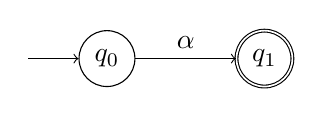
\begin{tikzpicture}
        \node[draw, circle] (A) at (0,0) {$q_0$};
        \draw[->] (-1,0) -- (A);
        \node[draw,circle,double] (B) at (2,0) {$q_1$};
        \draw[->] (A) -- (B);
        \draw (1,0) node [above] {$\alpha$};
     \end{tikzpicture}
     \rule{17cm}{0.5pt}\\
     \vspace{0.5cm}
     \caption{Automate reconnaissant $\alpha$ uniquement.}
     \label{fig:automate2}
 \end{figure}

 Nous allons maintenant prouver le sens réciproque. Pour cela, nous allons introduire une nouvelle classe d'automates, que l'on va appeler automates généralisés, dont les transitions seront étiquetées par des expressions rationnelles.

 \begin{defi}[Automate généralisé]
     Un automate généralisé est un automate dont la fonction de transition est définie par $\delta : \mathrm{Rat}(\Sigma)\times Q \to Q$ et qui ne possède qu'un état final. Un mot $u$ est accepté s'il peut être décomposé en $u_0\cdot u_1\cdots u_p$ et qu'il existe une suite $q_0,\ldots,q_{p+1}$ avec $q_{p+1}$ final et pour tout $i\leq p$, il existe $e\in\mathrm{Rat}(\Sigma)$ telle que $\delta(e,q_i)=q_{i+1}$ et $u_i\in L(e)$. De plus, on impose que $\delta$ n'est pas définie depuis $q_f$ l'état final et que $q_0$ n'est pas dans l'image de $\delta$.
 \end{defi}

 \begin{exo}
     Montrer que ces automates ont la même expressivité que les autres automates finis.
 \end{exo}

 \begin{rmk}
     Grâce à cet exercice, on peut supposer que pour tout automate $\aA$ il existe un automate généralisé $\aA'$ qui reconnaît le même langage.
 \end{rmk}

On va maintenant procéder sur l'automate généralisé en supprimant des transitions et des états jusqu'à n'obtenir qu'une seule transition, dont le label sera l'expression rationnelle associée à l'automate.

\begin{lem}[Réduction des transitions]
    Soit $\aA$ un automate généralisé, alors s'il existe $e,e'$ deux expressions et un état $q$ tels que $\delta(e,q)=\delta(e',q)$ alors on a un automate équivalent en supprimant ces deux transitions et en ajoutant $\delta(e+e',q)$.
\end{lem}

\begin{proof}
    Un mot reconnu par $\aA$ dont le chemin de lecture utilise $\delta(e,q)$ utilisera de la même façon $\delta(e+e',q)$, et réciproquement si un chemin de lecture utilise $\delta(e+e',q)$ alors soit le mot $u$ associé à cette transition est dans $L(e)$, auquel cas $\delta(e,q)$ donnera un chemin de lecture valide, soit il est dans $L(e')$ et $\delta(e',q)$ sera utilisé.
\end{proof}

On peut représenter cette réduction de la façon suivante :

\begin{figure}[htb]
    \centering
    \rule{17cm}{0.5pt}\\
    \vspace{0.5cm}
    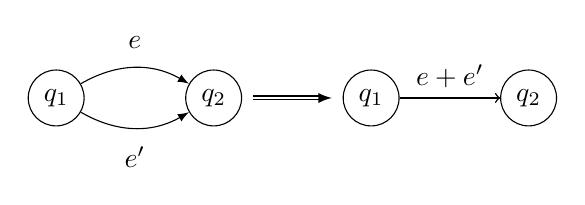
\begin{tikzpicture}
        \node[draw,circle] (A) at (-3,0) {$q_1$};
        \node[draw,circle] (B) at (-1,0) {$q_2$};
        \draw[->,>= latex] (A) to[bend left] (B);
        \draw[->,>= latex] (A) to [bend right] (B);
        \draw (-2,0.5) node [above] {$e$};
        \draw (-2,-0.5) node [below] {$e'$};
        \draw[->,>= latex, double distance = 1pt] (-0.5,0) -- (0.5,0);
        \node[draw,circle] (C) at (1,0) {$q_1$};
        \node[draw,circle] (D) at (3,0) {$q_2$};
        \draw[->,above] (C) -- (D);
        \draw[->,below] (C) -- (D);
        \draw (2,0) node [above] {$e+e'$};
    \end{tikzpicture}
    \rule{17cm}{0.5pt}\\
    \vspace{0.5cm}
    \caption{Réduction des transitions}
\end{figure}

\begin{lem}[\'Elimination des états]
    Soit un automate généralisé $\aA$ où l'on a réduit ses transitions, et $q$ un état ni initial ni final. Alors on peut construire un automate $\aA'$ reconnaissant le même langage en supprimant $q$ et, pour chaque couple d'états $(q_1,q_2)$ tel que $\delta(e_1,q_1)=q$ et $\delta(e_2,q)=q_2$, rajouter une transition de $q_1$ vers $q_2$ de la façon suivante :
    \begin{itemize}[label=$\bullet$]
        \item s'il existe $e$ telle que $\delta(e,q)=q$ alors on définit $\delta(e_1\cdot e^* \cdot e_2,q_1)=q_2$
        \item sinon, on définit $\delta(e_1\cdot e_2,q_1)=q_2$
    \end{itemize}
\end{lem}

\begin{proof}
    Dans le cas où le chemin de lecture ne passe pas par $q$, le lemme est évident. Supposons que dans la suite d'états $q_0,\ldots,q_p$ lisant un mot $u$ dans $\aA$ se trouve $q$, alors soit $q_1$ le prédécesseur de $q$ et $q_2$ son successeur (supposons d'abord que $q_2 \neq q$), dans la suite d'états. On sait qu'il existe une expression $e_1$ et une expression $e_2$ telles que $\delta(e_1,q_1)=q$ et $\delta(e_2,q)=q_2$ avec $u_1,u_2$ des parties du mot $u$ tels que $u_i\in L(e_i)$. Par définition, $u_1\cdot u_2\in L(e_1\cdot e_2)$ donc la suite d'états sans $q$ est valide dans $\aA$. Si jamais $q_2=q$, alors on peut remplacer toutes les suites de $q$ contiguës en disant que la transition est étiquetée par $e^*$ avec $e$ l'expression étiquetant la transition de $q$ à $q$.

    La réciproque est laissée en exercice au lecteur.
\end{proof}

On peut voit l'élimination d'états de la façon suivante :

\begin{figure}[htb]
    \centering
    \rule{17cm}{0.5pt}\\
    \vspace{0.5cm}
    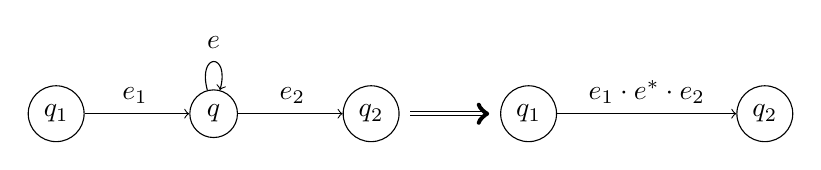
\begin{tikzpicture}
        \node[draw,circle] (A) at (-3,0) {$q$};
        \node[draw,circle] (B) at (-1,0) {$q_2$};
        \node[draw,circle] (E) at (-5,0) {$q_1$};
        \draw[->] (A) -- (B);
        \draw[->] (E) -- (A);
        \draw[->] (A) to[loop above] (A) ;
        \draw (-4,0) node [above] {$e_1$};
        \draw (-3,0.7) node [above] {$e$};
        \draw (-2,0) node [above] {$e_2$};
        \draw[->, double distance = 1pt] (-0.5,0) -- (0.5,0);
        \node[draw,circle] (C) at (1,0) {$q_1$};
        \node[draw,circle] (D) at (4,0) {$q_2$};
        \draw[->] (C) -- (D);
        \draw (2.5,0) node [above] {$e_1\cdot e^*\cdot e_2$};
    \end{tikzpicture}
    \rule{17cm}{0.5pt}\\
    \vspace{0.5cm}
    \caption{\'Elimination des états}
\end{figure}

On en déduit le résultat suivant :

\begin{prop}\label{prop:kleene2}
    Pour un automate généralisé $\aA$ il existe un automate généralisé $\aA'$ lisant le même langage et n'ayant qu'un état initial et un état final, et une seule transition entre les deux : le langage lu par $\aA'$ est exactement $L(e)$ pour $e$ l'étiquette de sa seule transition.
\end{prop}

\begin{proof}
    Il suffit de raisonner par récurrence sur le nombre d'états en appliquant l'élimination des états, et en réduisant les transitions qui en découlent. La dernière partie est par définition de la reconnaissance d'un mot dans un automate généralisé.
\end{proof}

On en déduit le théorème de Kleene :

\begin{them}[Kleene]
    La classe des langages rationnels est exactement l'ensemble des langages reconnus par des automates finis.
\end{them}

\begin{proof}
    C'est une conséquence directe des propositions \ref{prop:kleene1} et \ref{prop:kleene2}.
\end{proof}

\subsection{Myhill-Nérode}

Cette sous-section va s'attarder à une autre caractérisation des langages rationnels. Celle-ci est plus théorique mais présente plus facilement les limites des langages rationnels, et permet de répondre directement à la question \og y a-t-il pour un langage donné, un plus petit automate acceptant ce langage ?\fg{}

Tout d'abord, présentons un lemme en général utilisé pour montrer que des langages ne sont pas rationnels :

\begin{lem}[De l'étoile]
    Soit un langage rationnel $L$, alors il existe un nombre $M$ tel que pour tout mot $u\in L$ de longueur supérieure à $M$, il existe $v,w,x$ des mots ($w\neq\varepsilon$ mais les deux autres peuvent être vides) tels que $u = v\cdot w\cdot x$ et pour tout $n\in \nat$, $v\cdot w^n\cdot x \in L$. L'idée derrière est que pour les mots assez grands, il existe une partie du mot qui peut être répétée en restant dans le langage.
\end{lem}

\begin{proof}
    L'argument est principalement combinatoire : supposons que $u\in L$ avec $|u| > |Q|$ pour $Q$ l'ensemble d'états d'un automate $\aA$ reconnaissant $L$, alors lors de la lecture de $u$, on a la suite $q_0,\ldots,q_{|u|-1}$ et par principe des tiroirs, on trouve $i< j < |u|$ tels que $q_i = q_j$. On décompose alors le mot $u$ avec la partie préfixe $v := u_{<i}$, la partie infixe $w := u_{i,\ldots,j-1}$ et la partie postfixe $x := u_{j,\ldots,|u|-1}$. Dans ce cas, la lecture du mot $v\cdot w^n\cdot x$ donnera une suite d'états $q_0,\ldots,q_i$ puis $n$ fois la suite d'états de $q_i$ à lui-même décrite par $w$, puis la suite d'états $q_j,\ldots,q_{|u|-1}$  qui est un état final par hypothèse.
\end{proof}

\begin{rmk}
    Ce lemme est utile pour un langage infini : pour un langage fini, la constante sera simplement supérieure au cardinal du langage. De plus, la constante $M$ de ce lemme semble dépendre de l'automate reconnaissant le langage $L$, ce qui n'est pas naturel : le théorème de cette sous-section nous donnera justement une constante $M$ optimale et dépendant directement de $L$.
\end{rmk}

\begin{exo}
    En utilisant le lemme de l'étoile, montrer que le langage $\{0^n1^n\mid n\in\nat\}$ n'est pas rationnel.
\end{exo}

La notion principale pour pouvoir analyser les langages rationnels est celle de séparation des mots. L'idée derrière est simple : prenons deux mots $u$ et $v$, on peut les étendre naturellement en leur ajoutant un mot $z$ par concaténation, donnant $u\cdot z$ et $v\cdot z$. Dans ce cas, peut-on avoir un mot $z$ qui mène, depuis $u$, à un mot de $L$, et depuis $v$ à un mot qui n'est pas dans $L$ ? Cette notion motive notre prochaine définition :

\begin{defi}[Résiduel d'un langage]
    Soit $x$ un mot, on dénote par $x^{-1}L$ l'ensemble $$x^{-1}L=\{u\in \Sigma^*\mid x\cdot u \in L\}$$ appelé le résiduel de $L$ par $x$.

    De façon équivalente, on peut définir la relation d'équivalence d'inséparabilité : $x\sim y$ lorsque pour tout mot $u\in \Sigma^*$, $x\cdot u \in L \iff y\cdot u \in L$. Les classes d'équivalence pour cette relation sont les résiduels.
\end{defi}

Plusieurs observations s'ensuivent :
\begin{itemize}[label=$\bullet$]
    \item $L=\varepsilon^{-1}L$
    \item pour tout automate sur un langage $L$ fixé on peut associer à chaque état $q$ un résiduel de $L$.
\end{itemize}

Ces observations permettent d'imaginer les résiduels de $L$ comme un automate, lorsque le nombre de ses résiduels est fini. Le théorème de Myhill-Nérode stipule justement que ce nombre de résiduels est fini si et seulement si $L$ est rationnel.

\begin{them}[Myhill-Nérode]
    Soit $L$ un langage, alors $L$ est rationnel si et seulement s'il n'existe qu'un nombre fini de résiduels de $L$.
\end{them}

\begin{proof}
    Avec les observations antérieures, en supposant qu'il n'existe qu'un nombre fini de résiduels, on construit l'automate $\aA$ suivant :
    \begin{itemize}[label=$\bullet$]
        \item $Q = \{x^{-1}L\mid x \in \Sigma^*\}$
        \item $q_0 = \varepsilon^{-1}L$
        \item $\delta(\alpha,x^{-1}L) = (x\cdot \alpha)^{-1}L$ (la fonction est bien définie car si $x\sim y$ alors $x\cdot\alpha \sim y\dot\alpha$)
        \item $x^{-1}L$ est final s'il contient $\varepsilon$.
    \end{itemize}

    Si $x\in L$, alors $x^{-1}L$ contient $\varepsilon$ par construction, et s'il existe une suite d'états $q_0,\ldots,q_p$ menant à un état final dans cet automate, alors le dernier état est de la forme $x^{-1}L$ pour $x$ le mot lu et $\varepsilon\in x^{-1}L$ donc $x\cdot\varepsilon\in L$, c'est-à-dire $x\in L$. $L$ est donc reconnu par cet automate.

    Supposons que $L$ est rationnel. Alors soit $\aA$ un automate reconnaissant $L$. Pour chaque état $q$, on peut définir l'ensemble des mots menant de $q_0$ à $q$ : notons-le $P_q$. Alors pour deux mots $u,v\in P_q$, si $u\cdot z \in L$ alors $v\cdot z \in L$ car la lecture en partant de $q$ et en lisant les lettres de $z$ mène à un état final. Donc pour chaque état $q$, $P_q\subseteq x^{-1}L$ pour un certain $x$ (dépendant de $q$). On en déduit qu'il y a plus d'états que de résiduels, et comme l'automate est fini, qu'il y a un nombre fini de résiduels.
\end{proof}

\begin{rmk}
    La construction avec les résiduels nous donne donc aussi un automate minimal au sens du cardinal pour reconnaître un langage donné. Ainsi le lemme de l'étoile peut se reformuler en remplaçant \og il existe $M$\fg{} en remplaçant directement $M$ par le nombre de résiduels de $L$.
\end{rmk}

\begin{exo}
    Redémontrer que le langage $\{0^n1^n\mid n\in\nat\}$ n'est pas rationnel, cette fois-ci en utilisant le théorème de Myhill-Nérode.
\end{exo}

\begin{exo}
    L'ensemble des langages rationnels est-il stable par complémentaire ? Par intersection ?
\end{exo}

\begin{exo}
    Le langage des codes binaires de nombres multiples de $6$ est-il rationnel ?
\end{exo}

\begin{exo}
    Si $L$ est un langage rationnel, est-ce que le langage $\overline L$ des mots de $L$ à l'envers est rationnel ? Le langage des palindromes (mots qui sont les mêmes à l'envers) est-il rationnel ?
\end{exo}

La théorie des automates finis est bien plus vaste que le survol proposé ici : on peut par exemple parler de l'extension de ces automates aux mots infinis avec les automates de Büchi, ou encore de la détermination de l'arithmétique de Presburger avec des automates (ce dernier sujet aurait tout à fait sa place dans cet ouvrage dédié à la logique, mais comme l'objectif de ce chapitre n'est pas de voir en détail les automates mais seulement de mener naturellement aux machines de Turing, nous en ferons l'impasse).

Cependant, le problème avec les automates reste toujours le même : leur absence de mémoire et leur traitement purement linéaire de l'information. Le contre-exemple classique nous le montre bien : on ne peut pas compter de façon arbitrairement grande une valeur.
